\documentclass{article}
\usepackage{adjustbox}
\usepackage{graphicx}
\usepackage{geometry}
\usepackage{dcolumn}
 \geometry{
 a4paper,
 total={170mm,257mm},
 left=10mm,
 top=10mm
 }
 
\begin{document}

\section*{App Usage Over Time}

\subsubsection*{Methodology}
For every respondent that was treated, i.e., asked to download Bebbo app, we note the time that they were asked to download the app in the survey. We then aggregate their app usage activity by the weeks since they downloaded the app to get weekly app usage activity for each respondent. Note that this includes respondents across both Serbia and Bulgaria and across both baseline and endline periods.
We create variables summarizing their activity using events logged in the app.

\begin{enumerate}
    \item Home opens - Number of times the home page was opened in the week
    \item Days used - Number of days in the week the respondents used the app
    \item Usage count - Number of app events logged for the respondents in the week
    \item Opened - Binary variable indicating if any \textit{'\_opened'} event was logged in the week
    \item Home opened - Binary variable indicating if any \textit{'Home\_opened'} event was logged in the week
\end{enumerate}

\begin{figure}
\subsubsection*{Home opens over lifetime}
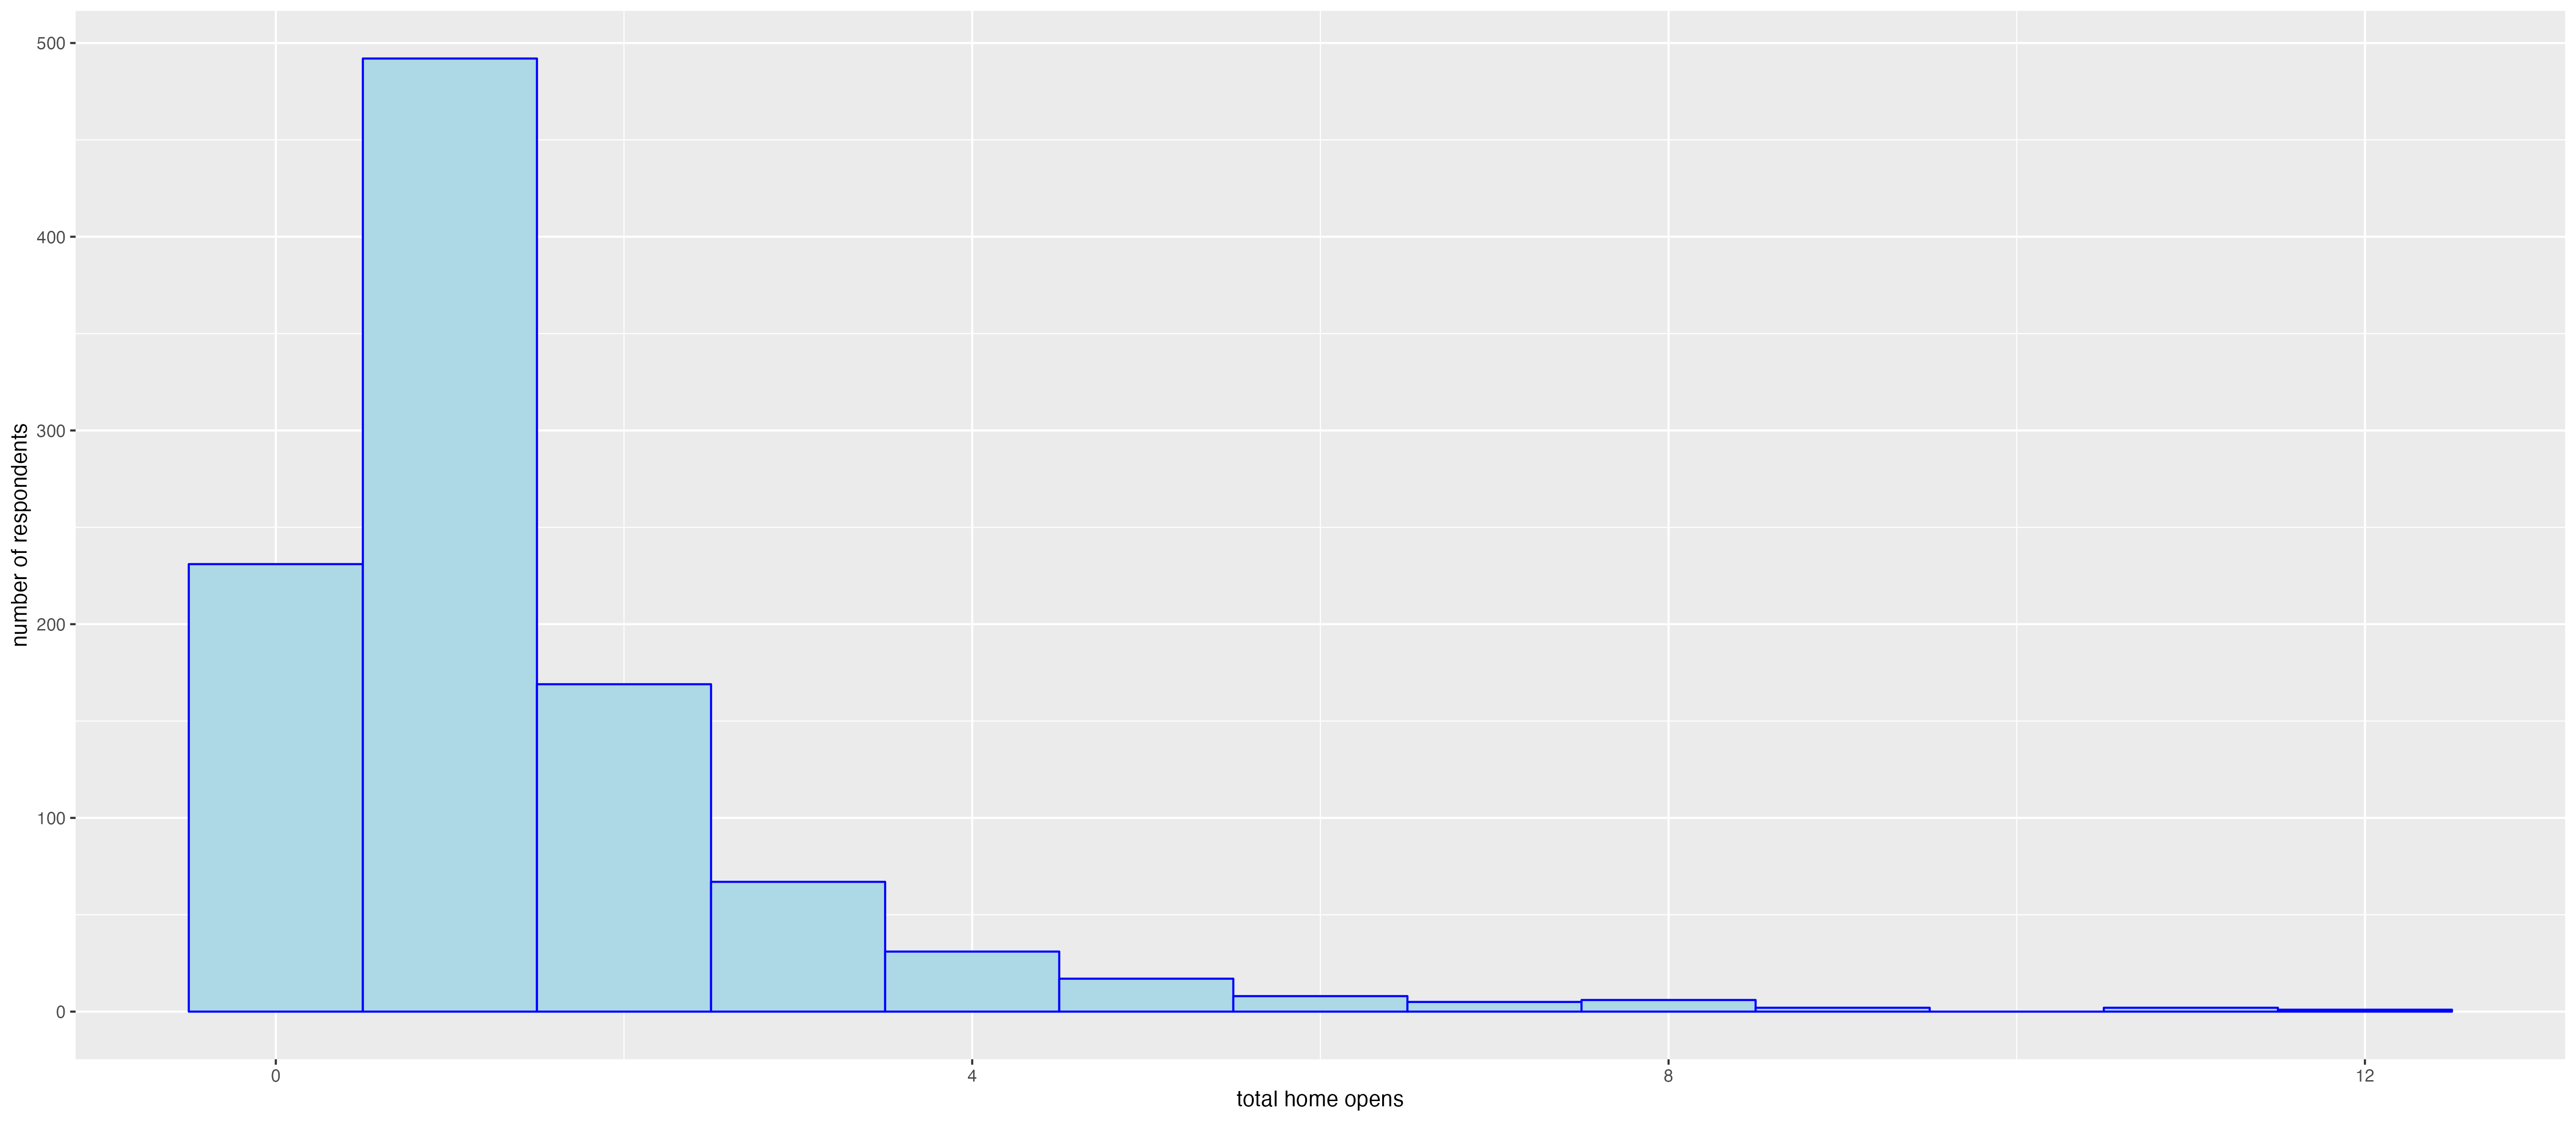
\includegraphics[scale=0.4]{app usage/plots/individual aggregates - home opens over lifetime.png}

\subsubsection*{Number of home opens over time}
The number of respondents who opened the app drops off steeply after week 1. 744 respondents filled had home open event logged in week 1 since treatment. 129 respondents had home open event logged in week 2. 
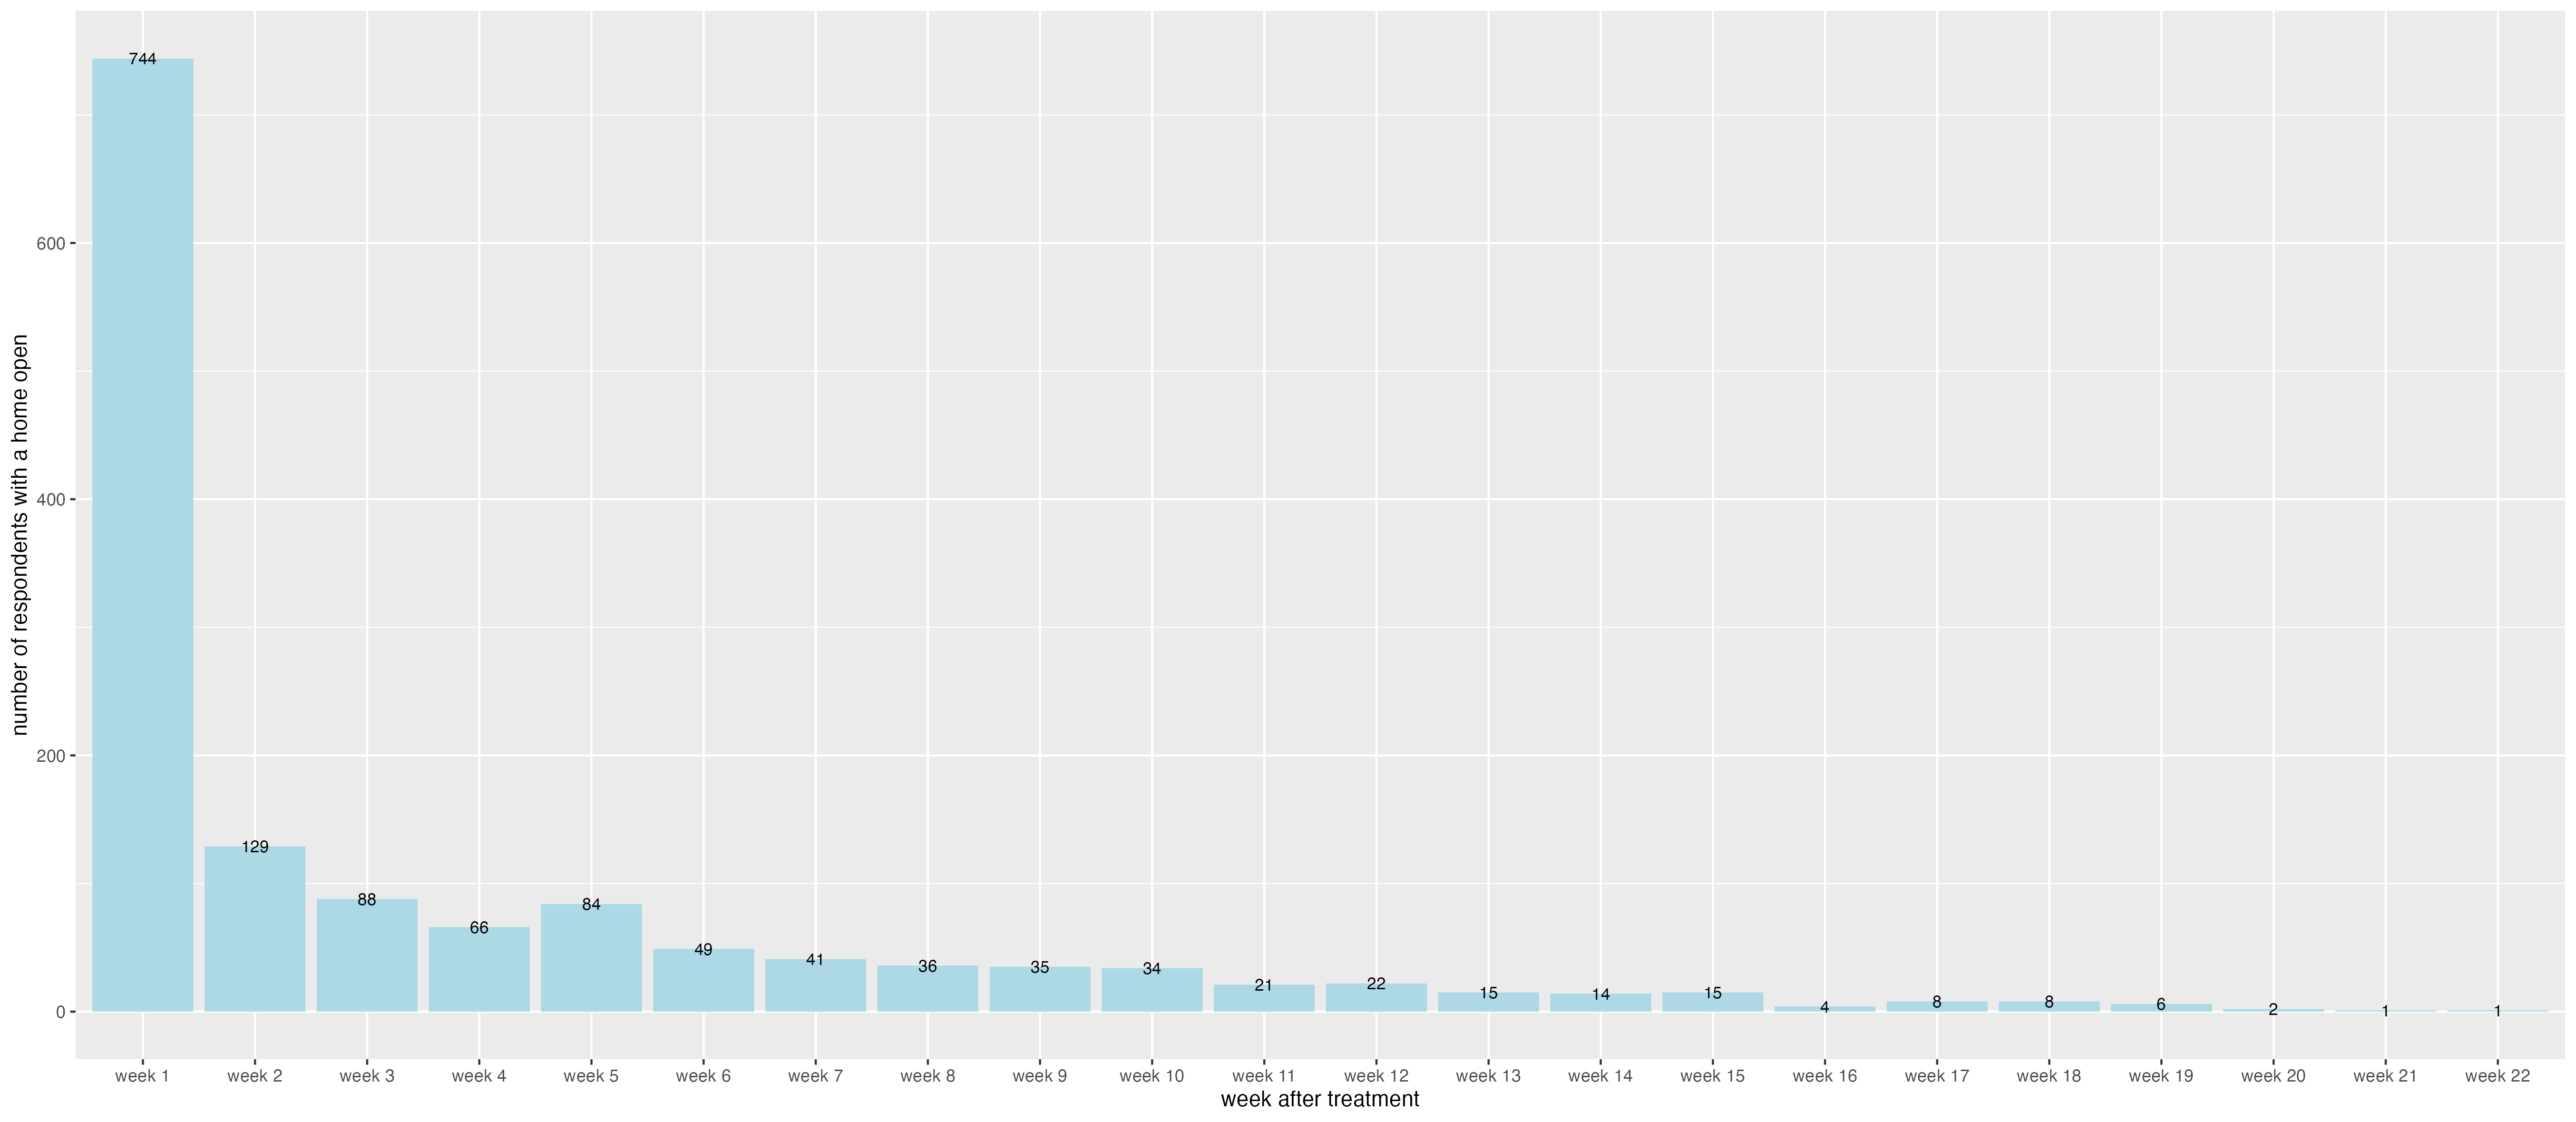
\includegraphics[scale=0.4]{app usage/plots/home opens over time - home opens.png}
\end{figure}

\begin{figure}
\subsubsection*{Number of days used}
We report the mean number of days of the week the respondent used the app. Respondents have app activity on 1 day in the week for most weeks. The text label annotates the number of respondents who opened any page of the app and contribute to the observations for that week. 
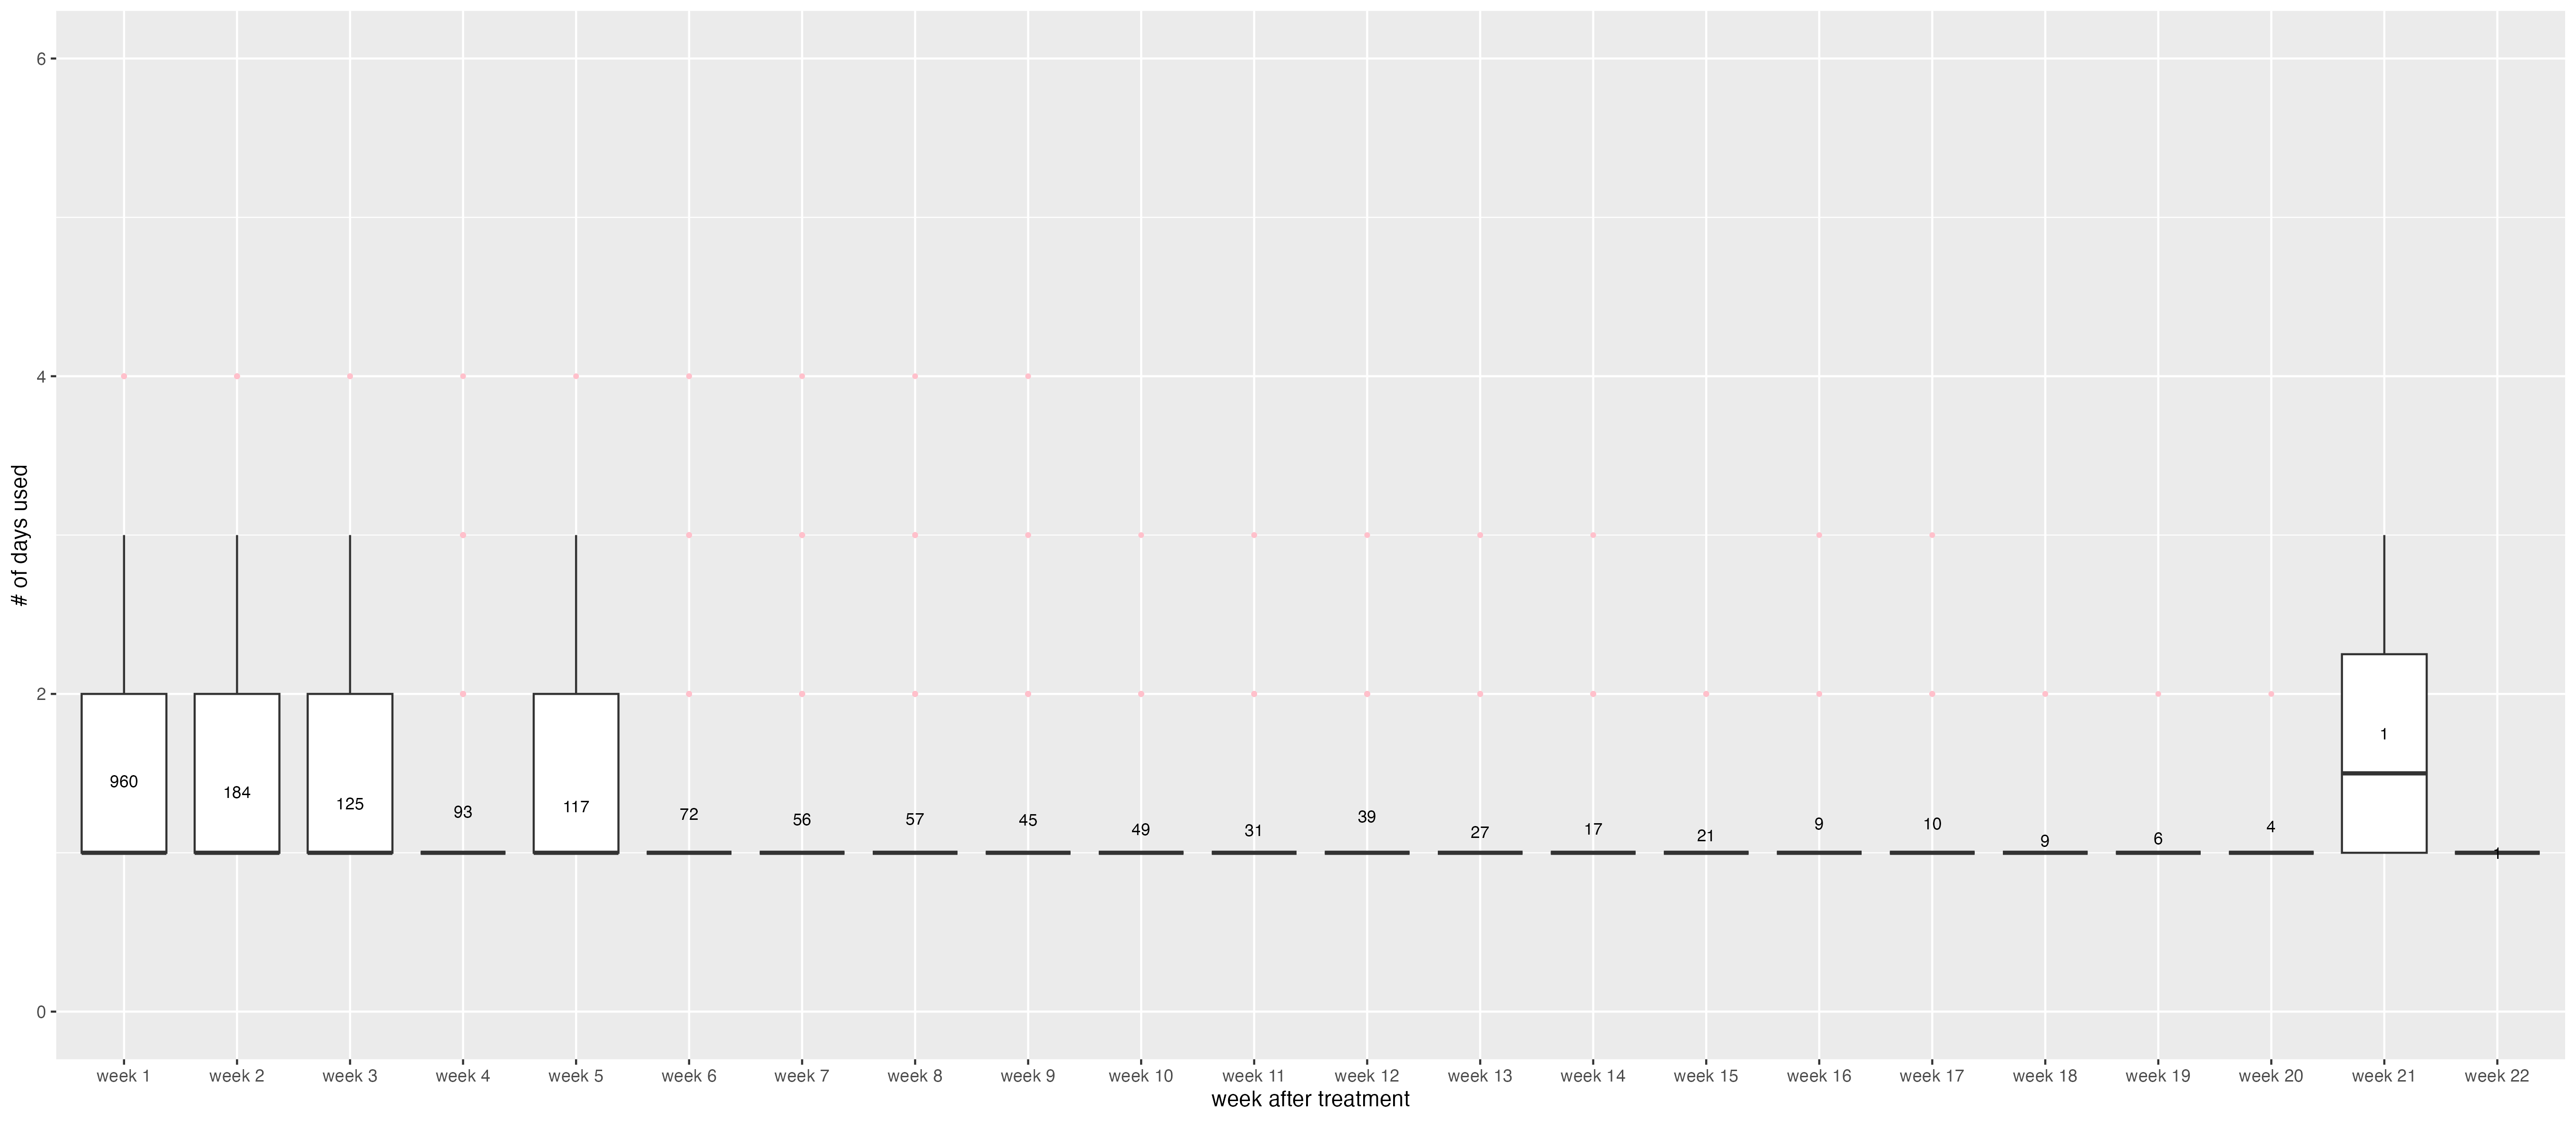
\includegraphics[scale=0.35]{plots/app usage over time - days used.png}

\subsubsection*{Usage counts}
We report the mean number of events logged for respondents for each week since treatment. The number of events logged drops steeply after week 1. The text label annotates the number of respondents who opened any page of the app and contributed to the observations for that week.
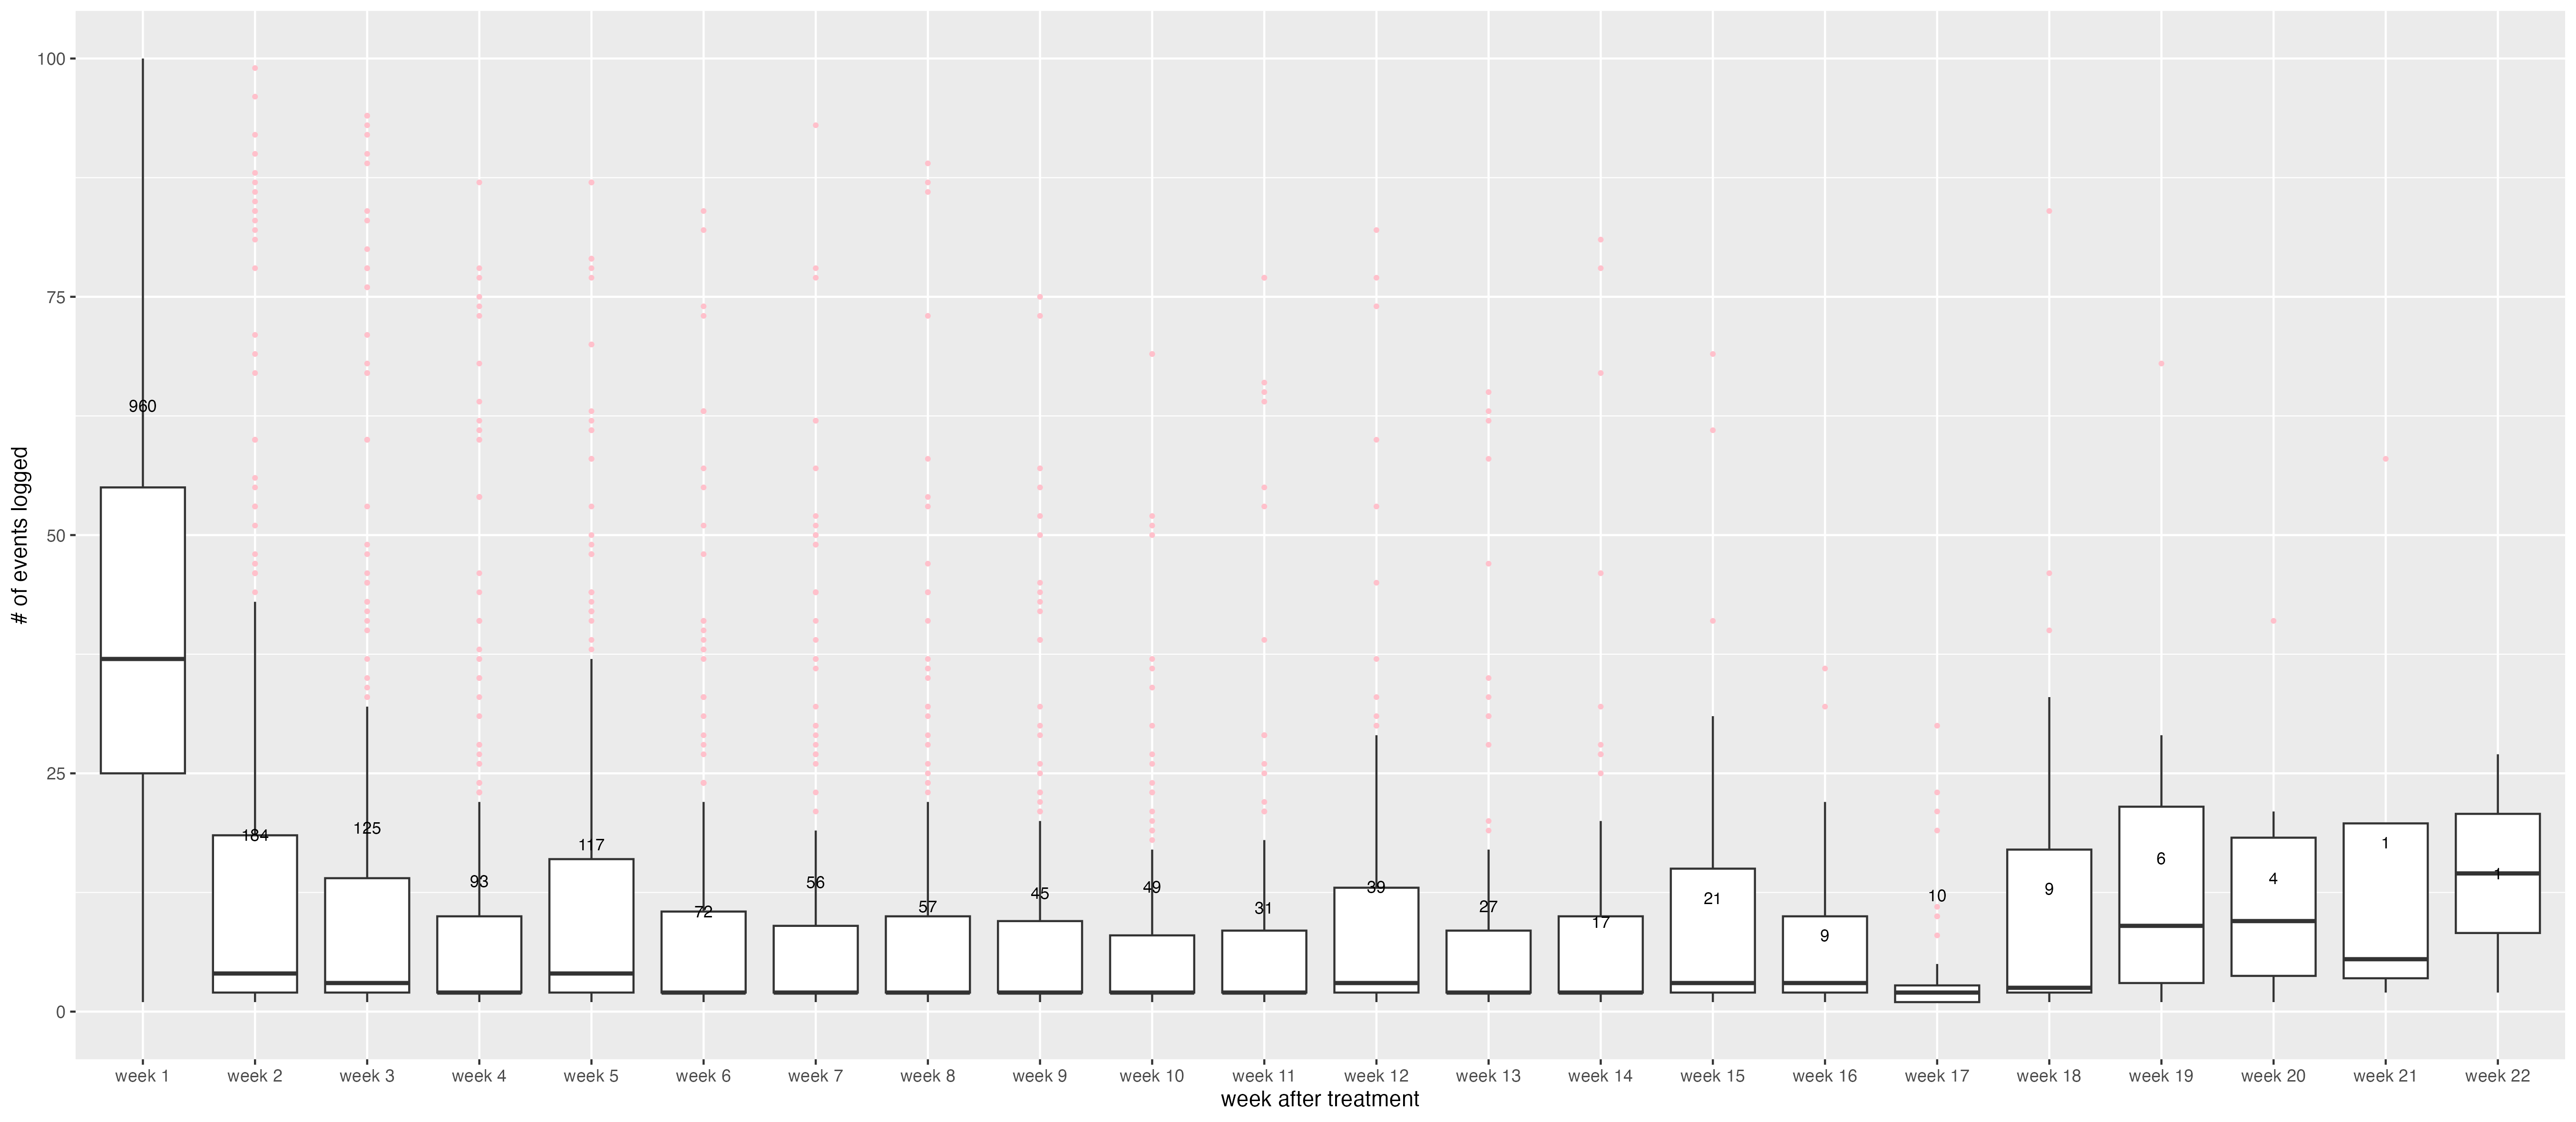
\includegraphics[scale=0.35]{plots/app usage over time - usage count.png}
\end{figure}

\begin{figure}
\subsubsection*{Home opens}
We report the mean number of home opens per respondent for each week since treatment. By week 4, the majority of respondents do not open the home page of the app except for some outliers. The text label annotates the number of respondents who opened any page of the app and contributed to the observations for that week.
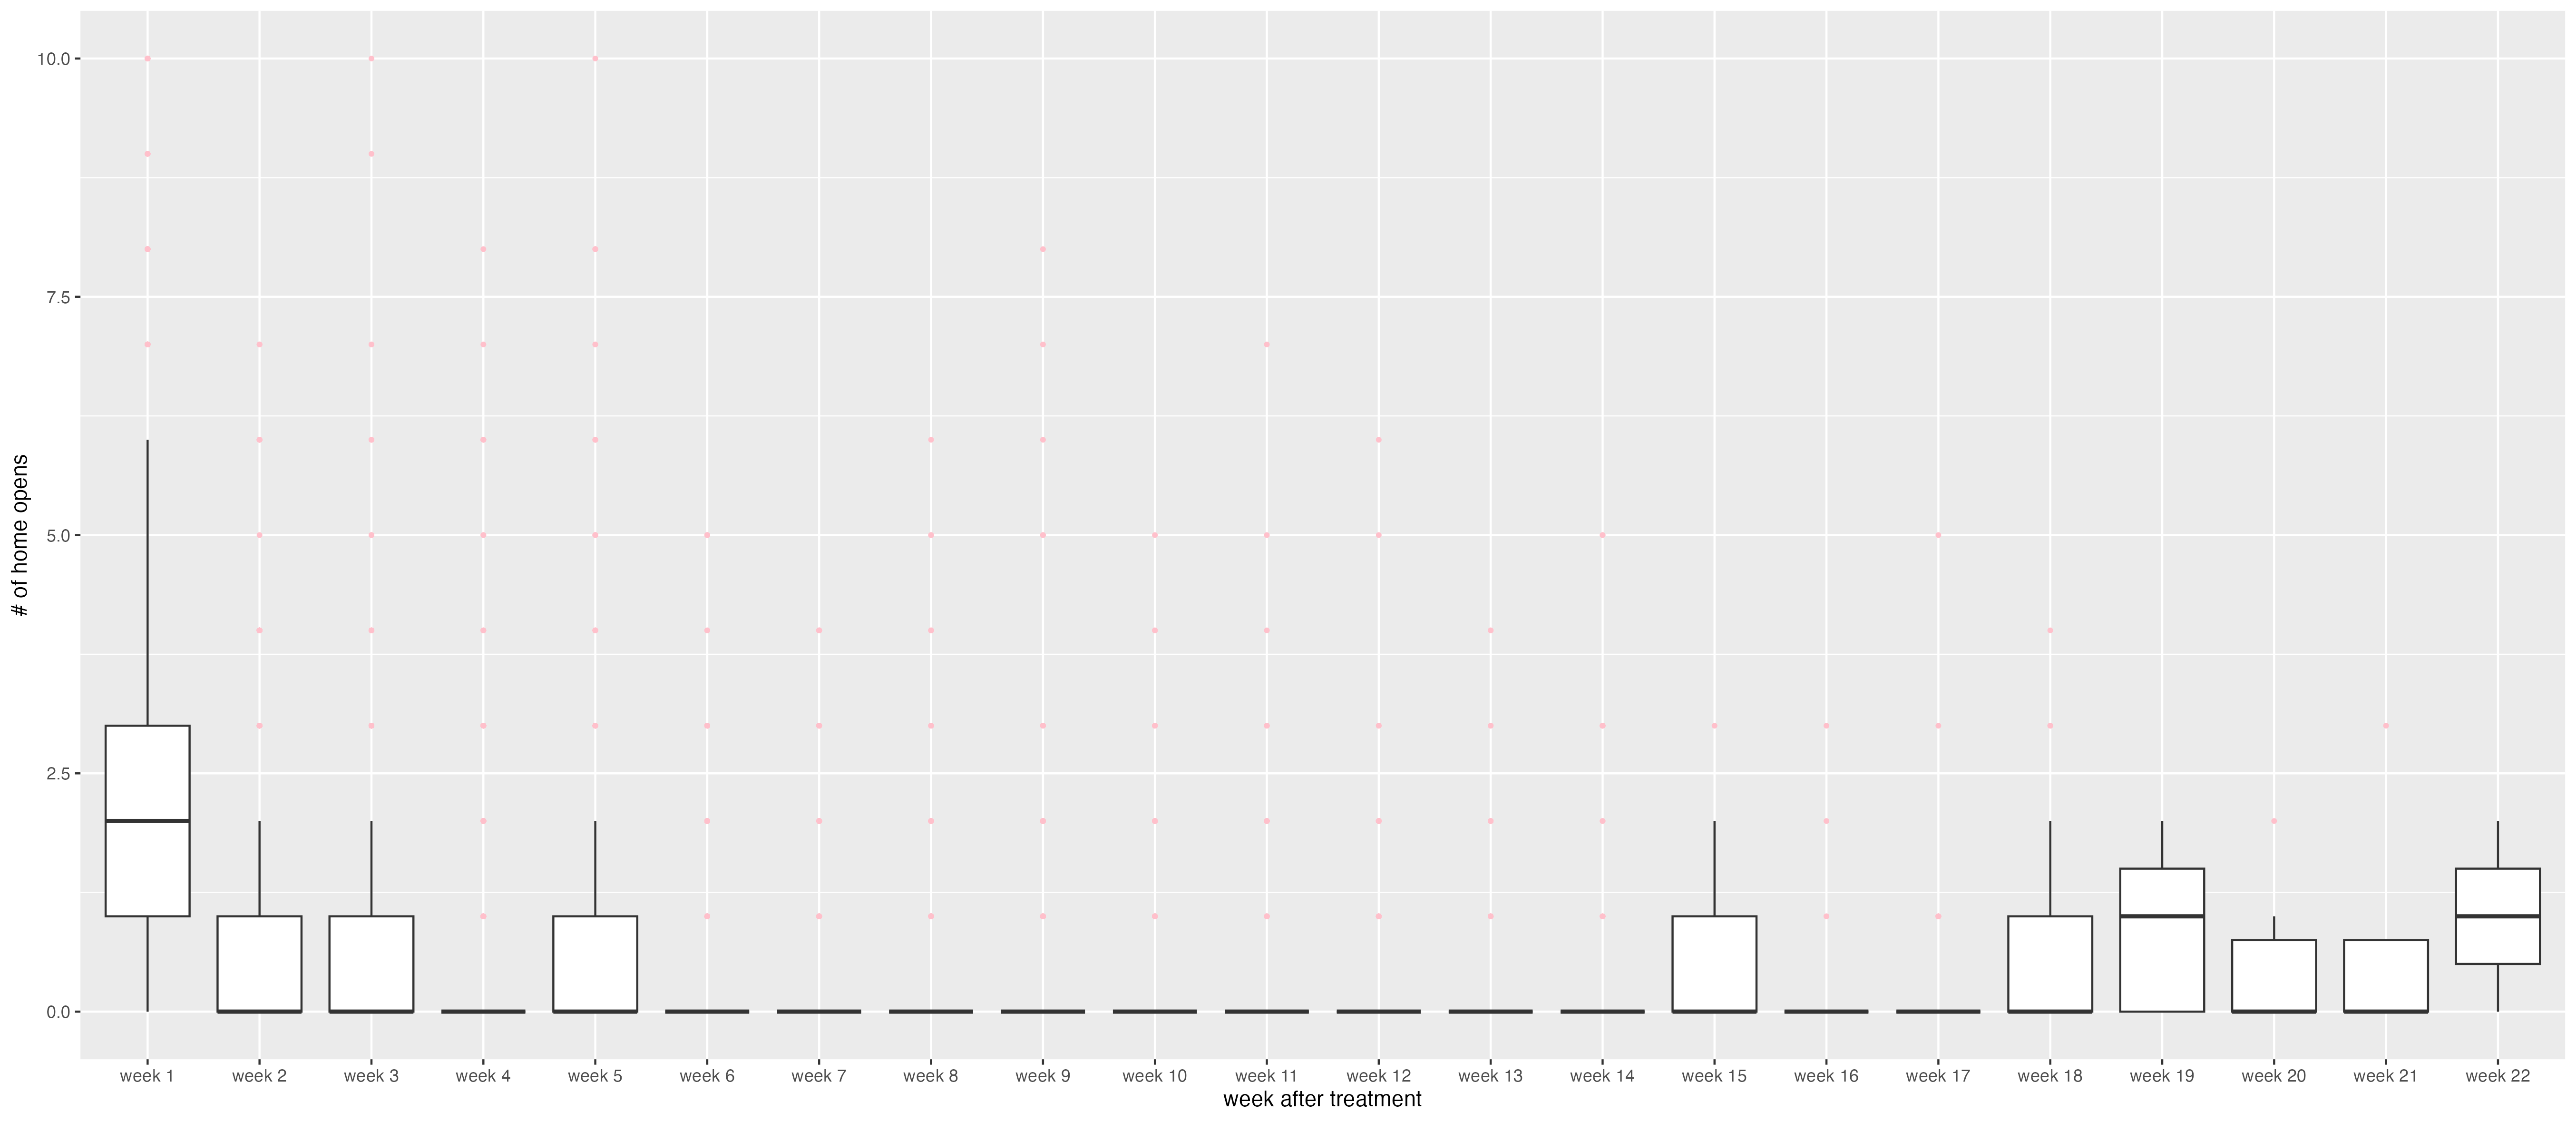
\includegraphics[scale=0.35]{plots/app usage over time - home opens.png}
\end{figure}

\section*{App Activity and User Characteristics}

In this analysis, we attempt to answer the questions - 
\begin{enumerate}
    \item Who are the respondents who used the app?
    \item Do more knowledgeable parents use the app more? 
\end{enumerate}

We do so by regressing respondents' app usage activity against their characteristics.
\vspace{1em}

\textbf{Independent variables :}
\begin{itemize}
    \item \textbf{Baseline characteristics} - respondents' scores on the construct variables. We only use the construct variables that have sufficiently high internal consistency. We drop the constructs that are highly correlated with other constructs. We find $parent\_knw$ to be correlated with $caregiver\_well\_being$. We drop the construct with lower reliability $caregiver\_well\_being$. 
    \item Demographics variables - parents' age flag (categorical), university flag (binary), gender (categorical), and number of children (numeric)
    \item Survey response variables - survey duration, start week, country flag
\end{itemize}

\textbf{Dependent variables :}
\begin{itemize}
    \item Home opened - binary variable indicating whether the respondent had a home opened event logged
    \item Home opens - continuous count variable indicating the respondents' count of total home opens
\end{itemize}
    
\subsubsection*{Home Opens and User Characteristics}
For respondents who downloaded the app, we regress their number of home opens against their baseline characteristics, demographic variables, and survey response variables. The adjusted $R^{2}$ for this model is 0.049. Note that the country flag is not significant which means that app usage does not differ significantly across the two countries after holding constant user characteristics.

% Table created by stargazer v.5.2.3 by Marek Hlavac, Social Policy Institute. E-mail: marek.hlavac at gmail.com
% Date and time: Mon, Sep 11, 2023 - 08:05:02
\begin{table}[!htbp] \centering 
  \caption{} 
  \label{tbl:app usage and baseline characteristics - linear reg} 
\begin{tabular}{@{\extracolsep{5pt}} ccccc} 
\\[-1.8ex]\hline 
\hline \\[-1.8ex] 
 & Estimate & Std. Error & t value & Pr(\textgreater \textbar t\textbar ) \\ 
\hline \\[-1.8ex] 
(Intercept) & $9.65$ & $1.66$ & $5.83$ & $0$ \\ 
start\_week & $$-$0.14$ & $0.04$ & $$-$4.16$ & $0$ \\ 
dev\_knw\_recog & $0.14$ & $0.59$ & $0.24$ & $0.81$ \\ 
attitude & $$-$0.11$ & $0.22$ & $$-$0.51$ & $0.61$ \\ 
caregiver\_well\_being & $$-$1.14$ & $0.31$ & $$-$3.66$ & $0$ \\ 
self\_care & $$-$0.12$ & $0.43$ & $$-$0.27$ & $0.79$ \\ 
family\_care & $0.11$ & $0.36$ & $0.31$ & $0.76$ \\ 
practices\_agree & $0.26$ & $0.26$ & $1.00$ & $0.32$ \\ 
practices\_hostility & $0.34$ & $0.26$ & $1.28$ & $0.20$ \\ 
parent\_age & $$-$0.02$ & $0.02$ & $$-$1.14$ & $0.25$ \\ 
number\_children & $0$ & $0$ & $0.49$ & $0.62$ \\ 
parent\_genderPrefer not to answer & $2.32$ & $1.55$ & $1.49$ & $0.14$ \\ 
parent\_genderWoman & $0.68$ & $0.46$ & $1.47$ & $0.14$ \\ 
survey\_duration & $0$ & $0$ & $1.28$ & $0.20$ \\ 
education & $0.02$ & $0.35$ & $0.05$ & $0.96$ \\ 
age\_flag2-6 & $$-$1.38$ & $0.34$ & $$-$4.06$ & $0$ \\ 
countryserbia & $$-$0.30$ & $0.58$ & $$-$0.51$ & $0.61$ \\ 
\hline \\[-1.8ex] 
\end{tabular} 
\end{table} 


\subsubsection*{Home Opened and User Characteristics}
For respondents who were treated, i.e., asked to download the Bebbo app, we fit a logistic regression model to whether the respondent had a home opened event logged using the respondents' baseline characteristics, demographic variables, and their survey response variables. The goodness of fit measure used is the percentage improvement in deviance over the null deviance (pseudo $R^{2}$). The pseudo $R^{2}$ for this model is 0.0299.

% Table created by stargazer v.5.2.3 by Marek Hlavac, Social Policy Institute. E-mail: marek.hlavac at gmail.com
% Date and time: Thu, Sep 21, 2023 - 00:32:36
\begin{table}[!htbp] \centering 
  \caption{home opened (binary) predicted by baseline characteristics} 
  \label{tbl:home opened and baseline characteristics - logistic reg} 
\begin{tabular}{@{\extracolsep{5pt}} ccccc} 
\\[-1.8ex]\hline 
\hline \\[-1.8ex] 
 & Estimate & Std. Error & z value & Pr(\textgreater \textbar z\textbar ) \\ 
\hline \\[-1.8ex] 
(Intercept) & $1.11$ & $0.52$ & $2.15$ & $0.03$ \\ 
start\_week & $$-$0.04$ & $0.01$ & $$-$3.87$ & $0$ \\ 
dev\_knw\_recog & $0.31$ & $0.17$ & $1.84$ & $0.06$ \\ 
confidence & $$-$0.15$ & $0.08$ & $$-$1.89$ & $0.06$ \\ 
attitude & $0.01$ & $0.06$ & $0.22$ & $0.82$ \\ 
caregiver\_well\_being & $$-$0.20$ & $0.09$ & $$-$2.12$ & $0.03$ \\ 
practices\_24 & $$-$0.62$ & $0.22$ & $$-$2.77$ & $0.01$ \\ 
practices\_agree & $0.13$ & $0.07$ & $1.84$ & $0.07$ \\ 
practices\_hostility & $$-$0.10$ & $0.07$ & $$-$1.44$ & $0.15$ \\ 
parent\_age & $$-$0.02$ & $0.01$ & $$-$3.71$ & $0$ \\ 
number\_children & $0$ & $0$ & $0.24$ & $0.81$ \\ 
parent\_genderWoman & $0.31$ & $0.13$ & $2.47$ & $0.01$ \\ 
survey\_duration & $0.06$ & $0.01$ & $4.59$ & $0$ \\ 
education & $0.11$ & $0.10$ & $1.12$ & $0.26$ \\ 
age\_flag2-6 & $0.11$ & $0.10$ & $1.15$ & $0.25$ \\ 
countryserbia & $0.20$ & $0.16$ & $1.29$ & $0.20$ \\ 
\hline \\[-1.8ex] 
\end{tabular} 
\end{table} 


\end{document}
